\documentclass[11pt,compress,t,notes=noshow, xcolor=table]{beamer}
\usepackage[]{graphicx}\usepackage[]{color}
% maxwidth is the original width if it is less than linewidth
% otherwise use linewidth (to make sure the graphics do not exceed the margin)
\makeatletter
\def\maxwidth{ %
  \ifdim\Gin@nat@width>\linewidth
    \linewidth
  \else
    \Gin@nat@width
  \fi
}
\makeatother

\definecolor{fgcolor}{rgb}{0.345, 0.345, 0.345}
\newcommand{\hlnum}[1]{\textcolor[rgb]{0.686,0.059,0.569}{#1}}%
\newcommand{\hlstr}[1]{\textcolor[rgb]{0.192,0.494,0.8}{#1}}%
\newcommand{\hlcom}[1]{\textcolor[rgb]{0.678,0.584,0.686}{\textit{#1}}}%
\newcommand{\hlopt}[1]{\textcolor[rgb]{0,0,0}{#1}}%
\newcommand{\hlstd}[1]{\textcolor[rgb]{0.345,0.345,0.345}{#1}}%
\newcommand{\hlkwa}[1]{\textcolor[rgb]{0.161,0.373,0.58}{\textbf{#1}}}%
\newcommand{\hlkwb}[1]{\textcolor[rgb]{0.69,0.353,0.396}{#1}}%
\newcommand{\hlkwc}[1]{\textcolor[rgb]{0.333,0.667,0.333}{#1}}%
\newcommand{\hlkwd}[1]{\textcolor[rgb]{0.737,0.353,0.396}{\textbf{#1}}}%
\let\hlipl\hlkwb

\usepackage{framed}
\makeatletter
\newenvironment{kframe}{%
 \def\at@end@of@kframe{}%
 \ifinner\ifhmode%
  \def\at@end@of@kframe{\end{minipage}}%
  \begin{minipage}{\columnwidth}%
 \fi\fi%
 \def\FrameCommand##1{\hskip\@totalleftmargin \hskip-\fboxsep
 \colorbox{shadecolor}{##1}\hskip-\fboxsep
     % There is no \\@totalrightmargin, so:
     \hskip-\linewidth \hskip-\@totalleftmargin \hskip\columnwidth}%
 \MakeFramed {\advance\hsize-\width
   \@totalleftmargin\z@ \linewidth\hsize
   \@setminipage}}%
 {\par\unskip\endMakeFramed%
 \at@end@of@kframe}
\makeatother

\definecolor{shadecolor}{rgb}{.97, .97, .97}
\definecolor{messagecolor}{rgb}{0, 0, 0}
\definecolor{warningcolor}{rgb}{1, 0, 1}
\definecolor{errorcolor}{rgb}{1, 0, 0}
\newenvironment{knitrout}{}{} % an empty environment to be redefined in TeX

\usepackage{alltt}
\newcommand{\SweaveOpts}[1]{}  % do not interfere with LaTeX
\newcommand{\SweaveInput}[1]{} % because they are not real TeX commands
\newcommand{\Sexpr}[1]{}       % will only be parsed by R



\usepackage[english]{babel}
\usepackage[utf8]{inputenc}

\usepackage{dsfont}
\usepackage{verbatim}
\usepackage{amsmath}
\usepackage{amsfonts}
\usepackage{bm}
\usepackage{csquotes}
\usepackage{multirow}
\usepackage{longtable}
\usepackage{booktabs}
\usepackage{enumerate}
\usepackage[absolute,overlay]{textpos}
\usepackage{psfrag}
\usepackage{algorithm}
\usepackage{algpseudocode}
\usepackage{eqnarray}
\usepackage{arydshln}
\usepackage{tabularx}
\usepackage{placeins}
\usepackage{tikz}
\usepackage{setspace}
\usepackage{colortbl}
\usepackage{mathtools}
\usepackage{wrapfig}
\usepackage{bm}
\usetikzlibrary{shapes,arrows,automata,positioning,calc,chains,trees, shadows}
\tikzset{
  %Define standard arrow tip
  >=stealth',
  %Define style for boxes
  punkt/.style={
    rectangle,
    rounded corners,
    draw=black, very thick,
    text width=6.5em,
    minimum height=2em,
    text centered},
  % Define arrow style
  pil/.style={
    ->,
    thick,
    shorten <=2pt,
    shorten >=2pt,}
}
\usepackage{subfig}


% Defines macros and environments

% basic latex stuff
\newcommand{\pkg}[1]{{\fontseries{b}\selectfont #1}} %fontstyle for R packages
\newcommand{\lz}{\vspace{0.5cm}} %vertical space
\newcommand{\dlz}{\vspace{1cm}} %double vertical space
\newcommand{\oneliner}[1] % Oneliner for important statements
{\begin{block}{}\begin{center}\begin{Large}#1\end{Large}\end{center}\end{block}}


%\usetheme{lmu-lecture}
\usepackage{../../style/lmu-lecture}

\let\code=\texttt
\let\proglang=\textsf

\setkeys{Gin}{width=0.9\textwidth}

\title{Introduction to Machine Learning}
% \author{Bernd Bischl, Christoph Molnar, Daniel Schalk, Fabian Scheipl}
\institute{\href{https://compstat-lmu.github.io/lecture_i2ml/}{compstat-lmu.github.io/lecture\_i2ml}}
\date{}

\setbeamertemplate{frametitle}{\expandafter\uppercase\expandafter\insertframetitle}



\begin{document}
% Set style/preamble.Rnw as parent.

% Load all R packages and set up knitr

% This file loads R packages, configures knitr options and sets preamble.Rnw as parent file
% IF YOU MODIFY THIS, PLZ ALSO MODIFY setup.Rmd ACCORDINGLY...








%! includes: basics-notation

\lecturechapter{ML-Basics: What is Machine Learning?}
\lecture{Introduction to Machine Learning}

\sloppy

% ------------------------------------------------------------------------------

\begin{frame}{Machine Learning}

Machine learning is a branch of statistics and computer science. 

\begin{center}

  \begin{figure}
    % 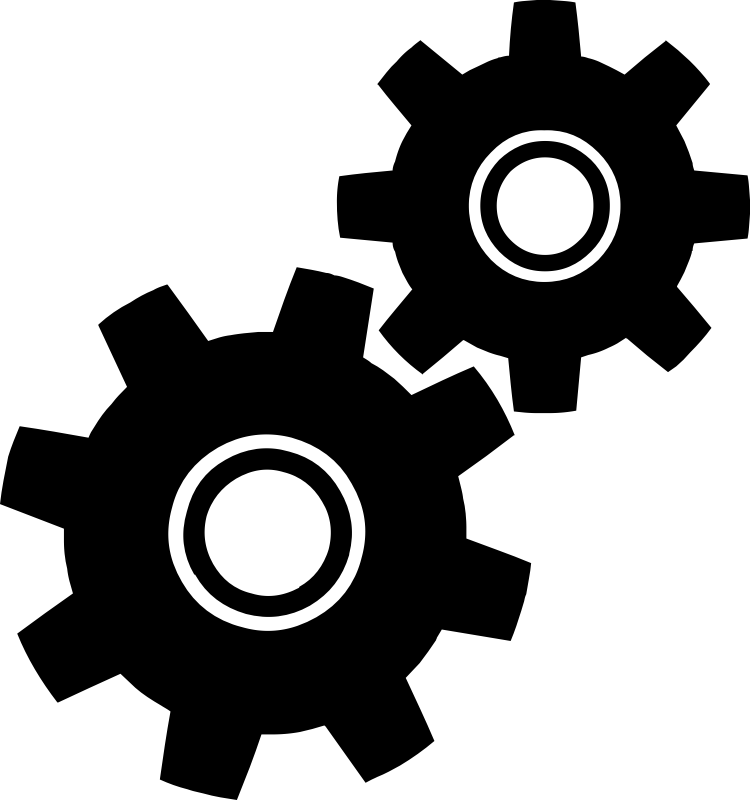
\includegraphics[width=0.4\textwidth]{figure_man/gears.png} \\
    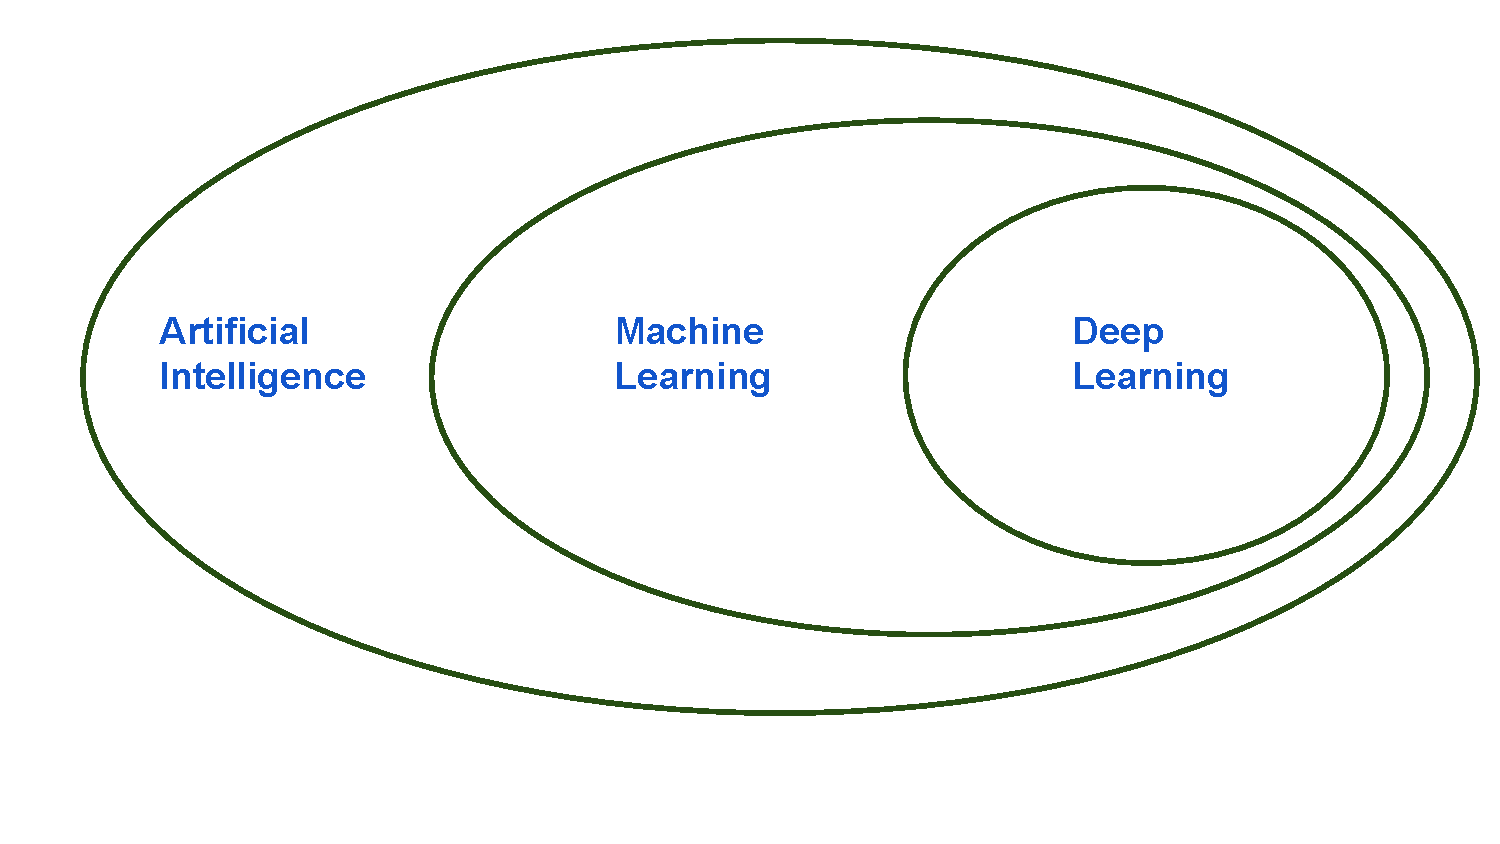
\includegraphics[width=0.7\textwidth]{figure_man/learning}
  \end{figure}

  \fontsize{13pt}{13pt}\selectfont
  
  % Machine Learning is a method of teaching computers to make predictions based 
  % on some data.

  A computer program is said to \textbf{learn} from experience E with respect to
  some task T and some performance measure P, if its performance on T, as 
  measured by P, improves with experience E. \\
  
  \begin{footnotesize}
  \emph{Tom Mitchell, Carnegie Mellon University, 1998}
  \end{footnotesize}
  
  \end{center}
  
\end{frame}

% ------------------------------------------------------------------------------

\begin{frame}{Machine Learning is changing our world}

\begin{itemize}

  \item Search engines learn what you want
  
  \item Recommender systems learn your taste in books, music, movies,...
  
  \item Algorithms do automatic stock trading
  
  \item Google Translate learns how to translate text
  
  \item Siri learns to understand speech
  
  \item DeepMind beats humans at Go
  
  \item Cars drive themselves
  
  % \item Medicines are developed faster
  
  \item Smart-watches monitor your health
  
  \item Election campaigns use algorithmically targeted ads to influence voters
  
  \item Data-driven discoveries are made in Physics, Biology, Genetics, 
  Astronomy, Chemistry, Neurology,...
  
  \item ...
  
\end{itemize}

\end{frame}

% ------------------------------------------------------------------------------

\begin{frame}{Coming up}

\begin{itemize}

  \item In this course, we focus on so-called \text{supervised ML}, in a 
  nutshell: using ML to predict something.
  
  \item In the first chapters, we will go through the fundamental terminology 
  and concepts in supervised ML which are relevant for everything that comes 
  next:
  
  \begin{itemize}
  
    \item What kind of "data" do we learn from?
    \item How can we formalize the goal of learning?
    \item What is a "prediction model"?
    \item How can we quantify "predictive performance"?
    \item What is a "learning algorithm" and how can we operationalize learning?
  
  \end{itemize}
  
  \item We will also look at a couple of fairly simple ML models to obtain a
  basic understanding and look at some concrete examples.
  
  \item More complex stuff comes later.
  
\end{itemize}

\end{frame}

% ------------------------------------------------------------------------------

\begin{frame}{Machine Learning Tasks}

\begin{center}
  % FIGURE SOURCE: No source available
  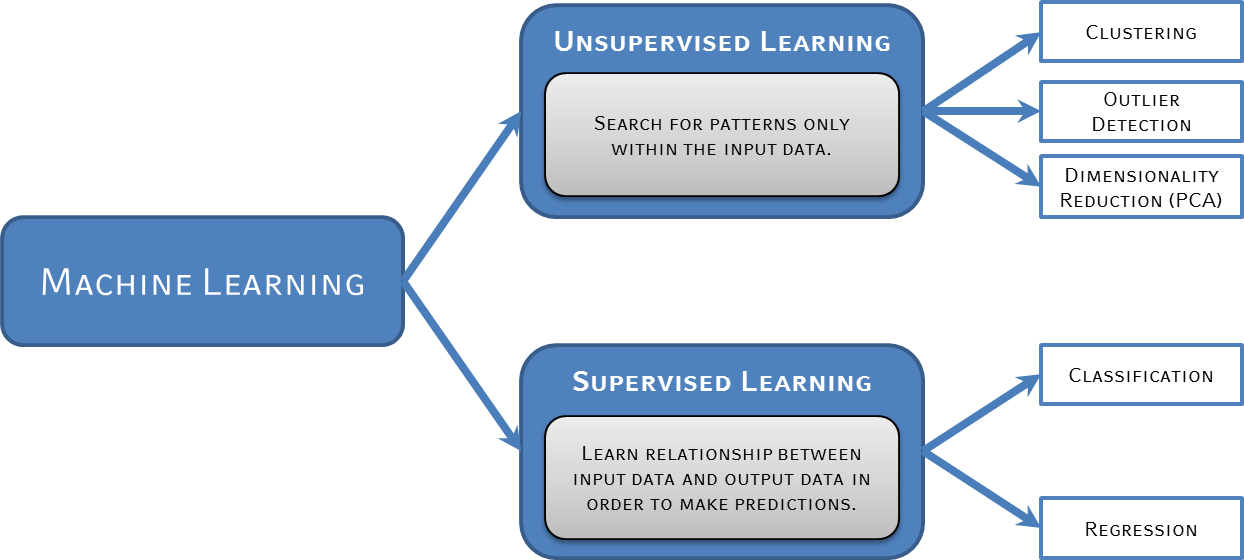
\includegraphics[height=0.5\textheight]{figure_man/ml-types.png}
\end{center}

In this course, we will deal with \textbf{supervised learning} for regression 
and classification only: predicting labels $y$ based on features $x$, using 
pattterns that we learned from labeled training data.

\end{frame}

% ------------------------------------------------------------------------------

% Jann's summary slide for all other learning tasks

\begin{vbframe}{Additional Learning Tasks}

\lz

\textbf{Unsupervised learning}

\begin{itemize}

  \item Data without labels $y$
  
  \item Search for patterns within the inputs $x$
  
  \item \textit{Unsupervised} as there is no external criterion to optimize or 
  \enquote{true} output
  
  \begin{itemize}
  
    \item Dimensionality reduction (PCA, Autoencoders ...): compress 
    information in $\mathcal X$
    
    \item Clustering: group similar observations, separate dissimilar 
    observations
    
    \item Outlier detection, anomaly detection
    
    \item Association rules
  
  \end{itemize}

\end{itemize}
    
\framebreak

\lz

\textbf{Semi-Supervised learning}

\begin{itemize}

  \item Large amount of labeled data necessary to train reliable model
  
  \item Creating labeled datasets often very expensive
  
  \item Learn from labeled (expensive) \textbf{and} unlabeled (cheap) data
  
  \item Unlabeled data in conjunction with a small amount of labeled data 
  improves learning accuracy

\end{itemize}
\lz
    \begin{figure}[!htb]
    %images from rcourses  
  \minipage{0.31\textwidth}
    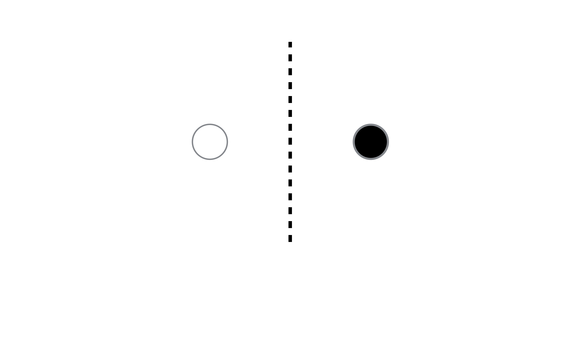
\includegraphics[width=\linewidth]{figure_man/semi1.png}
  \endminipage\hfill
  \minipage{0.31\textwidth}
    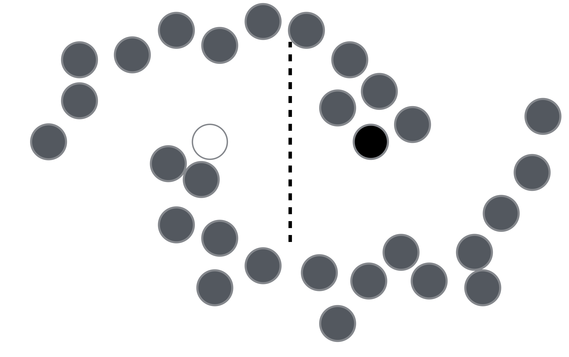
\includegraphics[width=\linewidth]{figure_man/semi3.png}
  \endminipage\hfill
  \minipage{0.31\textwidth}%
    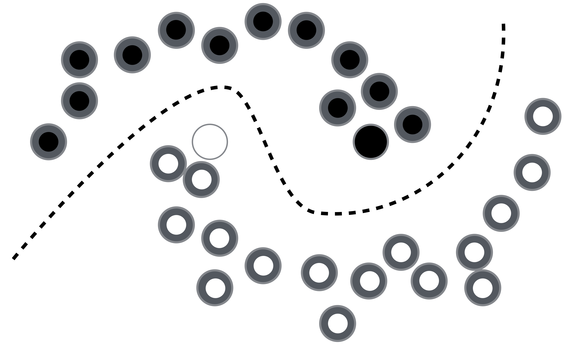
\includegraphics[width=\linewidth]{figure_man/semi7.png}
  \endminipage
  \end{figure}
\framebreak

\textbf{Reinforcement learning}

\begin{itemize}

  \item Select actions in subsequent  states within a certain environment to 
  maximize lagged future reward
  
  \item Example: train neural net to play mario kart (environment)
  
  \begin{itemize}
  
    \item Accelerate/ steer/ break (actions) at each time point (states) during 
    playing
    
    \item Reward: ranking after finish, should be maximized
  
  \end{itemize}

\end{itemize}

\begin{center}
  %image from rcourses
  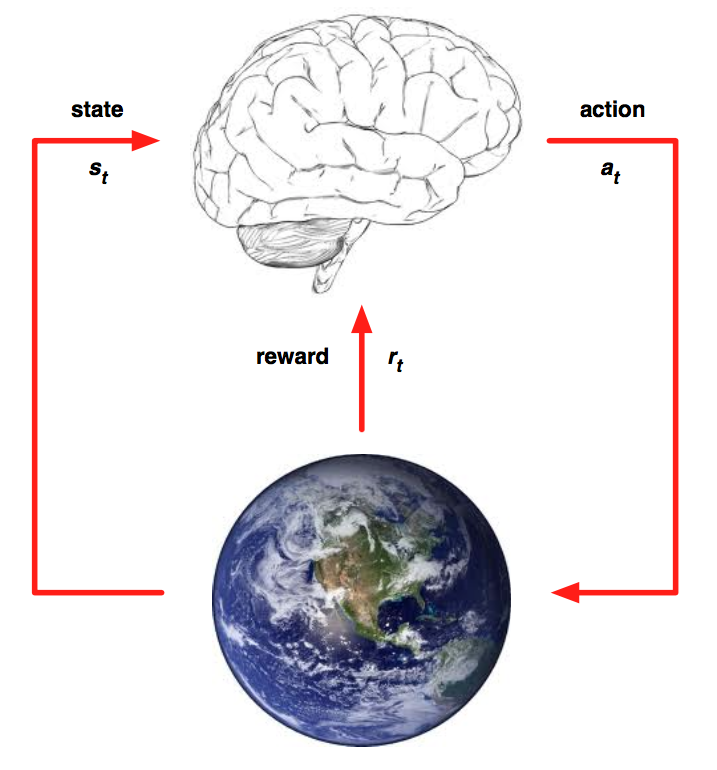
\includegraphics[height=0.45\textheight,keepaspectratio]{figure_man/state_action_reward_diagram.png}
\end{center}

\end{vbframe}

% ------------------------------------------------------------------------------

\endlecture
\end{document}
